% Practica 6 · Diagrama a bloques del sistema y del programa
% Optoelectronica V3736 · 2026B · Dr. Ruben Estrada Marmolejo
\documentclass[border=10pt]{standalone}
\usepackage[T1]{fontenc}
\usepackage[utf8]{inputenc}
\usepackage{lmodern}
\renewcommand{\familydefault}{\sfdefault}
\usepackage{tikz}
\usetikzlibrary{positioning,arrows.meta,calc,fit,backgrounds}
\definecolor{optosignal}{HTML}{2A5CAA}
\definecolor{optoemit}{HTML}{C9601F}
\definecolor{optoalert}{HTML}{B23A34}
\definecolor{optodetect}{HTML}{6B4C9A}
\definecolor{optoink}{HTML}{1C1F24}
\definecolor{optoconfirm}{HTML}{3E7C59}
\definecolor{optorule}{HTML}{D8DBE0}
\begin{document}
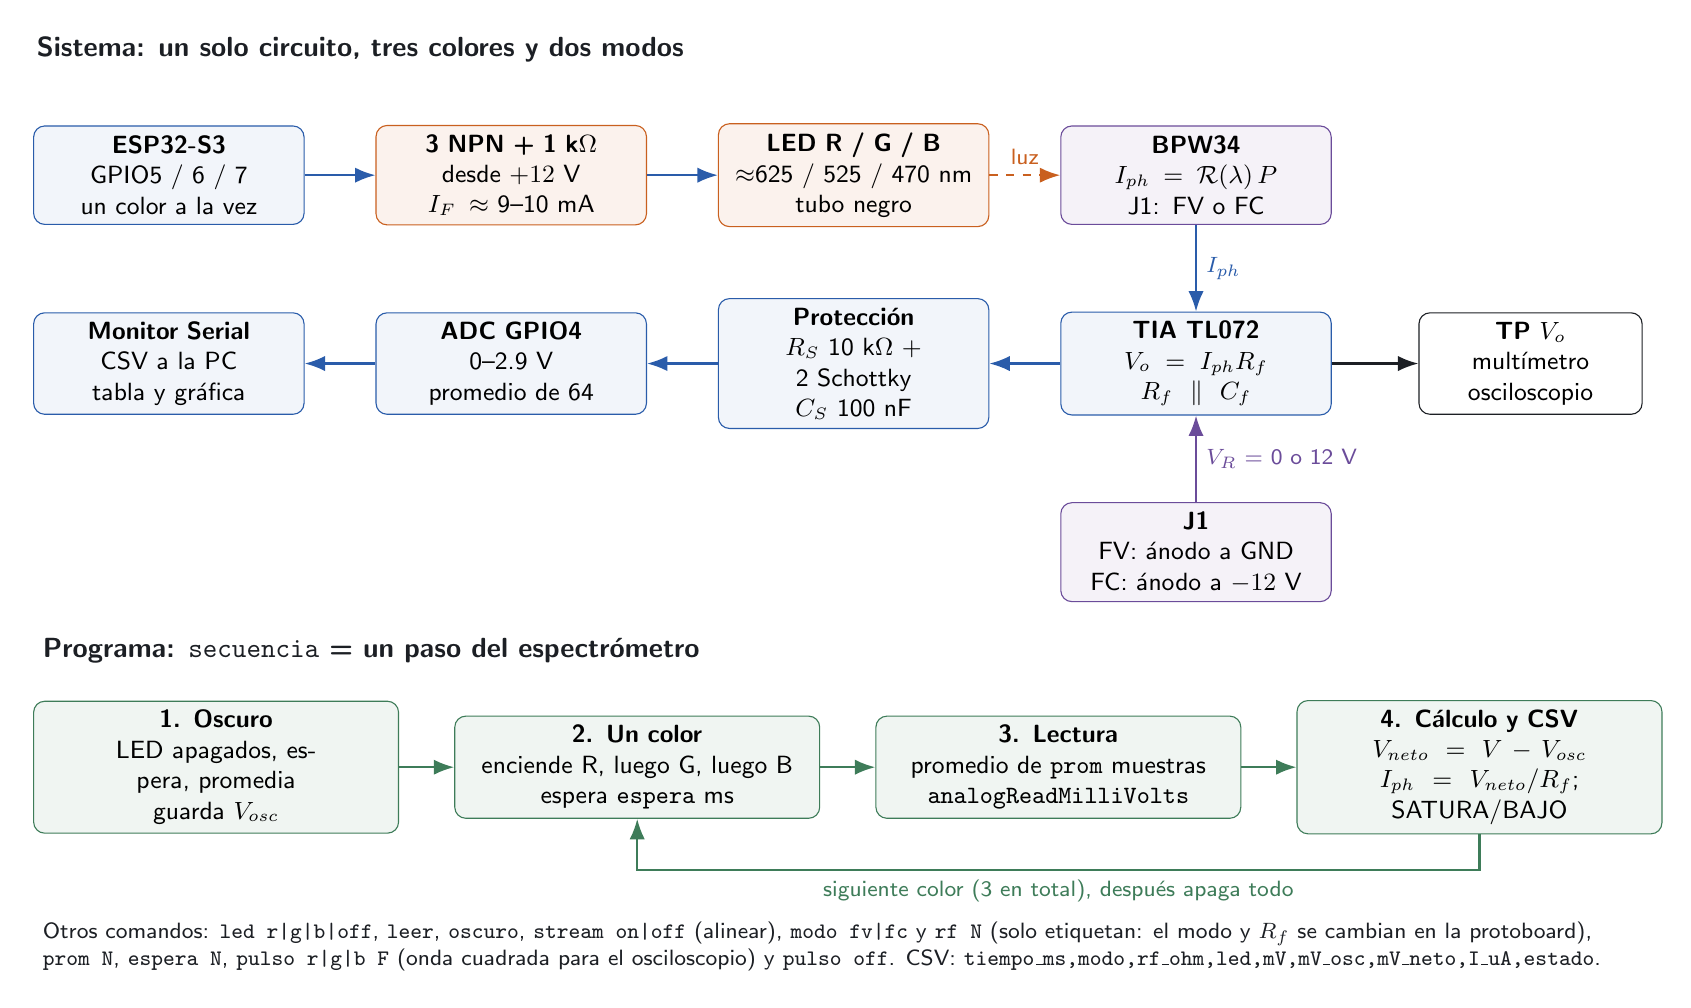
\begin{tikzpicture}[
  b/.style={draw=optosignal,rounded corners,fill=optosignal!6,align=center,minimum height=1.25cm,text width=3.2cm,font=\small},
  e/.style={b,draw=optoemit,fill=optoemit!8},
  d/.style={b,draw=optodetect,fill=optodetect!7},
  s/.style={b,draw=optoconfirm,fill=optoconfirm!8,text width=4.4cm},
  f/.style={-{Latex[length=2.6mm]},thick,optosignal},
  node distance=0.75cm and 0.9cm]
% ---------- Hardware ----------
\node[font=\bfseries,text=optoink,anchor=west] at (-1.8,1.6) {Sistema: un solo circuito, tres colores y dos modos};
\node[b] (esp) {\textbf{ESP32-S3}\\GPIO5 / 6 / 7\\un color a la vez};
\node[e,right=of esp] (drv) {\textbf{3 NPN + 1 k$\Omega$}\\desde $+12$ V\\$I_F\approx$ 9--10 mA};
\node[e,right=of drv] (led) {\textbf{LED R / G / B}\\$\approx$625 / 525 / 470 nm\\tubo negro};
\node[d,right=of led] (pd) {\textbf{BPW34}\\$I_{ph}=\mathcal{R}(\lambda)\,P$\\J1: FV o FC};
\node[b,below=1.1cm of pd] (tia) {\textbf{TIA TL072}\\$V_o=I_{ph}R_f$\\$R_f\parallel C_f$};
\node[b,left=of tia] (prot) {\textbf{Protección}\\$R_S$ 10 k$\Omega$ + 2 Schottky\\$C_S$ 100 nF};
\node[b,left=of prot] (adc) {\textbf{ADC GPIO4}\\0--2.9 V\\promedio de 64};
\node[b,left=of adc] (pc) {\textbf{Monitor Serial}\\CSV a la PC\\tabla y gráfica};
\node[d,below=1.1cm of tia,text width=3.2cm] (bias) {\textbf{J1}\\FV: ánodo a GND\\FC: ánodo a $-12$ V};
\node[b,right=1.1cm of tia,text width=2.6cm,draw=optoink,fill=white] (tp) {\textbf{TP $V_o$}\\multímetro\\osciloscopio};
\draw[f] (esp)--(drv); \draw[f] (drv)--(led);
\draw[f,optoemit,dashed] (led)--node[above,font=\footnotesize]{luz}(pd);
\draw[f] (pd)--node[right,font=\footnotesize]{$I_{ph}$}(tia);
\draw[f] (tia)--(prot); \draw[f] (prot)--(adc); \draw[f] (adc)--(pc);
\draw[f,optodetect] (bias)--node[right,font=\footnotesize]{$V_R$ = 0 o 12 V}(tia);
\draw[f,optoink] (tia)--(tp);
% ---------- Programa ----------
\node[font=\bfseries,text=optoink,anchor=west] at ($(pc.south west)+(0,-3.0)$) (tit) {Programa: \texttt{secuencia} = un paso del espectrómetro};
\node[s,below=0.35cm of tit.south west,anchor=north west] (p1) {\textbf{1. Oscuro}\\LED apagados, espera, promedia\\guarda $V_{osc}$};
\node[s,right=0.7cm of p1] (p2) {\textbf{2. Un color}\\enciende R, luego G, luego B\\espera \texttt{espera} ms};
\node[s,right=0.7cm of p2] (p3) {\textbf{3. Lectura}\\promedio de \texttt{prom} muestras\\\texttt{analogReadMilliVolts}};
\node[s,right=0.7cm of p3] (p4) {\textbf{4. Cálculo y CSV}\\$V_{neto}=V-V_{osc}$\\$I_{ph}=V_{neto}/R_f$; SATURA/BAJO};
\draw[f,optoconfirm] (p1)--(p2); \draw[f,optoconfirm] (p2)--(p3); \draw[f,optoconfirm] (p3)--(p4);
\draw[f,optoconfirm] (p4.south) -- ++(0,-0.45) -| node[pos=0.25,below,font=\footnotesize]{siguiente color (3 en total), después apaga todo} (p2.south);
\node[align=left,font=\footnotesize,text=optoink,anchor=north west] at ($(p1.south west)+(0,-1.0)$) {%
Otros comandos: \texttt{led r|g|b|off}, \texttt{leer}, \texttt{oscuro}, \texttt{stream on|off} (alinear), \texttt{modo fv|fc} y \texttt{rf N} (solo etiquetan: el modo y $R_f$ se cambian en la protoboard),\\
\texttt{prom N}, \texttt{espera N}, \texttt{pulso r|g|b F} (onda cuadrada para el osciloscopio) y \texttt{pulso off}. CSV: \texttt{tiempo\_ms,modo,rf\_ohm,led,mV,mV\_osc,mV\_neto,I\_uA,estado}.};
\end{tikzpicture}
\end{document}
